\documentclass{beamer}
\usepackage[T1]{fontenc}
\usepackage[utf8]{inputenc}
\usepackage[german]{babel}
\usepackage{graphicx}
\usepackage{subcaption}
\usepackage{bytefield}
\usepackage{mathtools}
\usepackage[all]{xy}

\usetheme{Warsaw}

\setbeamercolor{normal text}{fg=white,bg=black!90}
\setbeamercolor{structure}{fg=white}

\setbeamercolor{alerted text}{fg=red!85!black}

\setbeamercolor{item projected}{use=item,fg=black,bg=item.fg!35}

\setbeamercolor*{palette primary}{use=structure,fg=structure.fg}
\setbeamercolor*{palette secondary}{use=structure,fg=structure.fg!95!black}
\setbeamercolor*{palette tertiary}{use=structure,fg=structure.fg!90!black}
\setbeamercolor*{palette quaternary}{use=structure,fg=structure.fg!95!black,bg=black!80}

\setbeamercolor*{framesubtitle}{fg=white}

\setbeamercolor*{block title}{parent=structure,bg=black!60}
\setbeamercolor*{block body}{fg=black,bg=black!10}
\setbeamercolor*{block title alerted}{parent=alerted text,bg=black!15}
\setbeamercolor*{block title example}{parent=example text,bg=black!15}


\title{GPUDirect MPI Communications and Optimizations to Accelerate FFTs on Exascale Systems}
\subtitle{Seminararbeit im Masterstudium an der OTH Regensburg}
\author{Robert Graf, Tobias Seitz}

\begin{document}
\frame
{
	\titlepage
}

\frame
{
	\frametitle{Beispieltitel}
	BlaBlaBlubberBlubberFaselBlabla
	\begin{itemize}
		\item Erstens
		\item Zweitens
		\item Drittens
		\item etc.
	\end{itemize}
}

\frame
{
	\begin{center}
		\Large Kommunikationskostenoptimierung \normalsize
	\end{center}
}
\frame
{
	\frametitle{Motivation}
	\begin{figure}[h!]
		\centering
		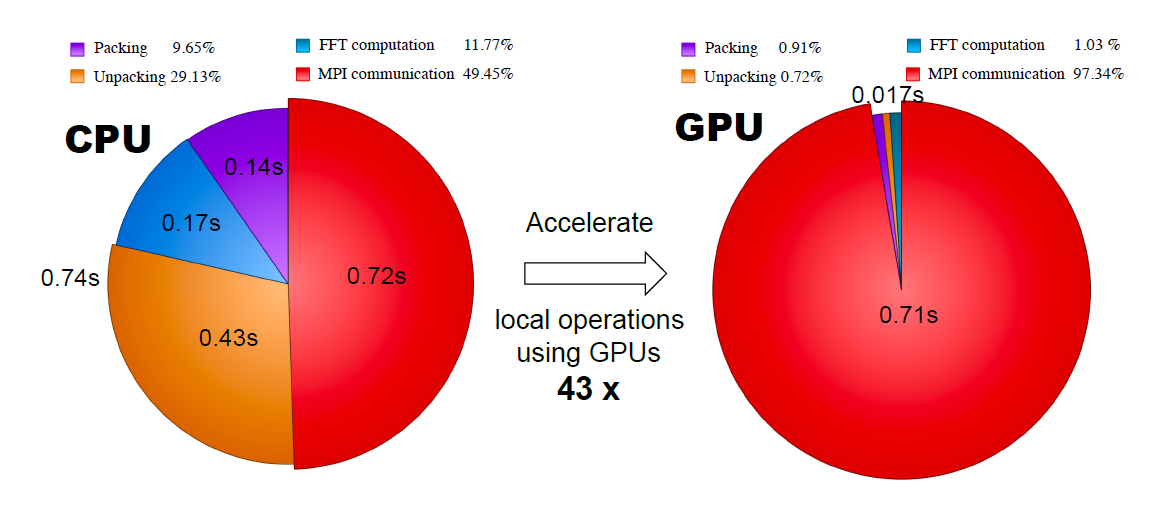
\includegraphics[width=\linewidth, keepaspectratio]{../res/speedup.png}
	\end{figure}
	\begin{itemize}
		\item $\frac{0.14s+0.17s+0.42s+0.72s}{0.017s+0.71s}=200,8\% \rightarrow$  2-fache Beschleunigung
		\item Kommunikationszeit nur vernachlässigbare Änderung
		\item rechte Seite graphisch nicht akkurat dargestellt!
	\end{itemize}
}
\frame
{
	\frametitle{Bottleneck: Kommunikation}
	Nach der Beschleunigung ist der  Zeitanteil der Kommunikation:\\
	$$\frac{0.71s}{0.71s+0.017}\approx97,6\%$$
	$\implies$ Bottleneck in der Kommunikation\\
	\large Was tun? \normalsize
}
\frame
{
	\frametitle{Was tun?}
	Konzeptionell 2 Ansätze:
	\begin{itemize}
		\item Option1: Verwendung eines besseren Algorithmus hinsichtlich serieller Anteile und Kommunikation.
		\item Option2: Verbesserung der Kommunikationsstrategie unter Einbeziehung von Eigenschaften der Systemarchitektur.
	\end{itemize}
}
\frame
{
	\frametitle{Systemarchitektur}
	\begin{figure}[h!]
		\centering
		\begin{subfigure}[t]{0.3\linewidth}
			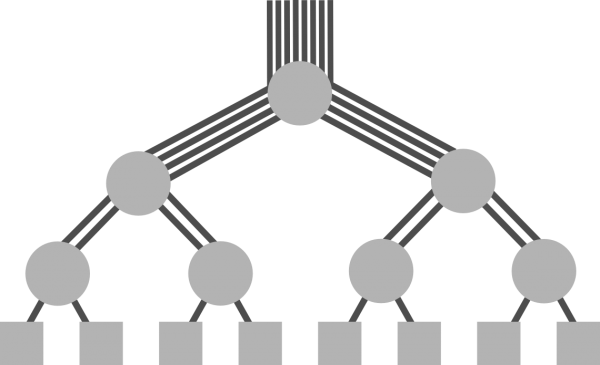
\includegraphics[width=1\linewidth]{../res/fat_tree.png}
			\footnotemark[1]
		\end{subfigure}
~
		\begin{subfigure}[t]{0.6\linewidth}
			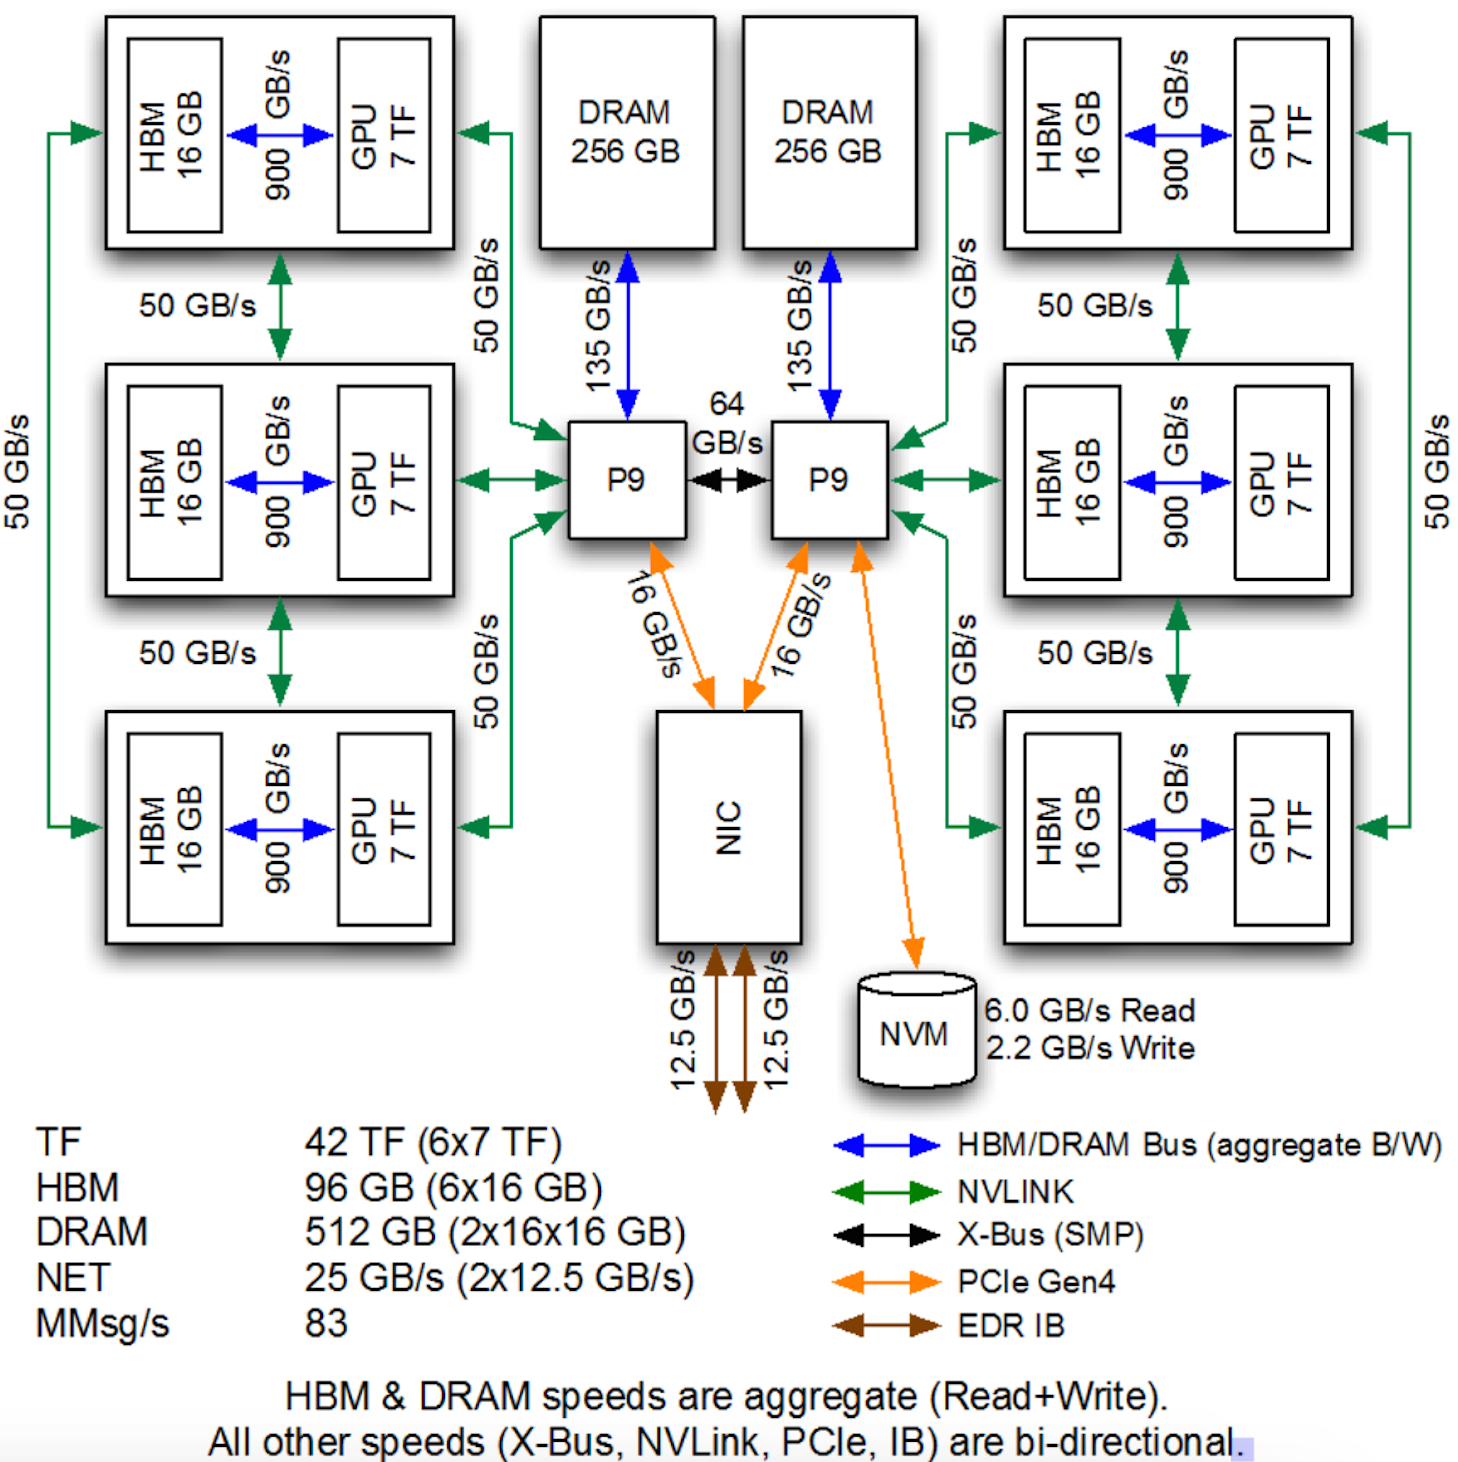
\includegraphics[width=1\linewidth]{../res/architecture.png}
			\footnotemark[2]
		\end{subfigure}
	\end{figure}

\footnotetext[1]{\tiny\url{https://clusterdesign.org/fat-trees/} am 6.2.2019\normalsize}
\footnotetext[2]{\tiny Shajek H., Tomov S., Ayala A., Haidar A., Dongarra J:\\{\sl GPUDirect MPI Communications and Optimizations to Accelerate FFTs on Exascale Systems};\\EuroMPI ’19 Posters, September 11-13, 2019, Zurich, Switzerland}
\normalsize
}
\frame
{
	\frametitle{Ansatz 0}
	Benchmarks zur Ermittlung der tatsächlichen Bandbreite.
	\begin{figure}[h!]
		\centering
		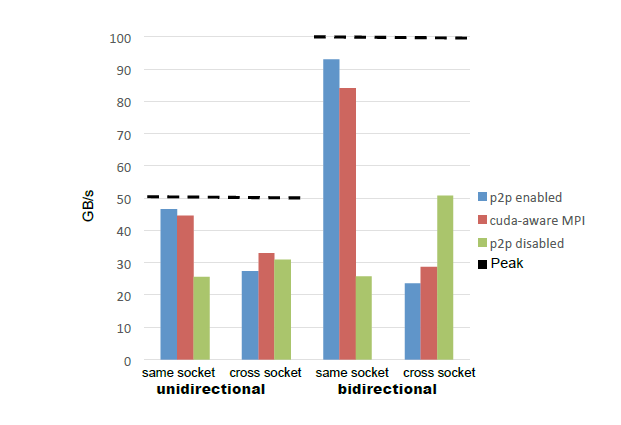
\includegraphics[width=0.7\linewidth, keepaspectratio]{../res/bench0.png}
	\footnotemark[1]
	\end{figure}
\footnotetext[1]{\tiny Shajek H., Tomov S., Ayala A., Haidar A., Dongarra J:\\{\sl GPUDirect MPI Communications and Optimizations to Accelerate FFTs on Exascale Systems};\\EuroMPI ’19 Posters, September 11-13, 2019, Zurich, Switzerland}
}
\frame
{
	\frametitle{Ansatz 1}
	Nach Option2: Untersuchung Kommunikativer Eigenschaften der Systemarchitektur
	\begin{figure}[h!]
		\centering
		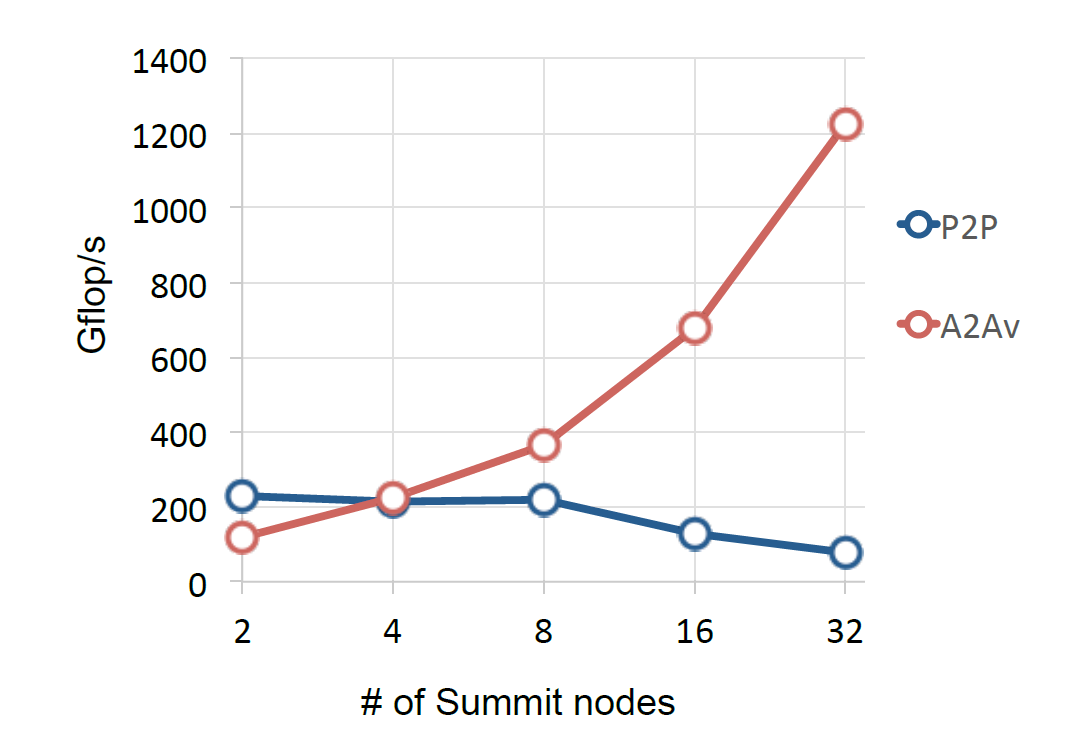
\includegraphics[width=0.7\linewidth, keepaspectratio]{../res/bench.png}
		\footnotemark[1]
	\end{figure}
\footnotetext[1]{\tiny Shajek H., Tomov S., Ayala A., Haidar A., Dongarra J:\\{\sl GPUDirect MPI Communications and Optimizations to Accelerate FFTs on Exascale Systems};\\EuroMPI ’19 Posters, September 11-13, 2019, Zurich, Switzerland}
}
\frame
{
	\frametitle{Ansatz 2}
	Nach Option1: Algorithmische Anpassung
	\begin{figure}[h!]
		\centering
		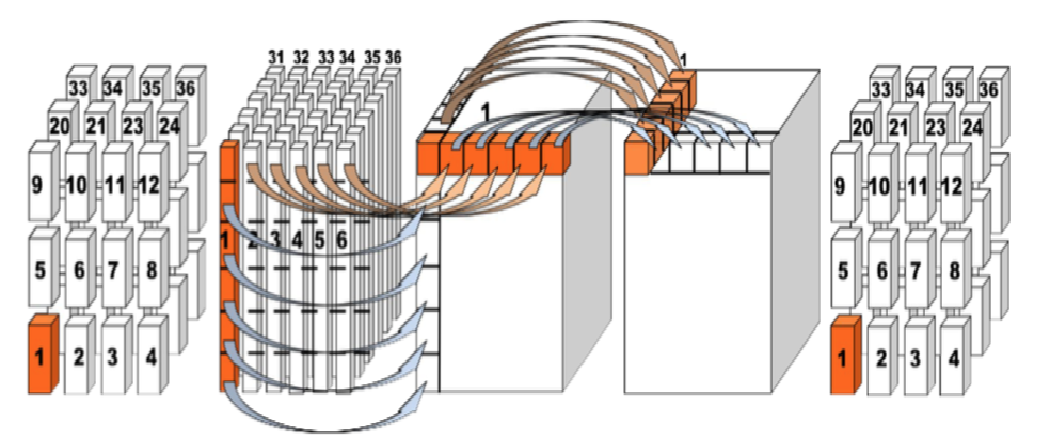
\includegraphics[width=0.7\linewidth, keepaspectratio]{../res/algo.png}
		\footnotemark[1]
	\end{figure}
	1D\textit{pencil} $\rightarrow$ 2D\textit{slabs} Übertragungsgröße
	$(TransformX,TransformY,TransformZ,MoveBack)\rightarrow(TransformY,TransformZ,MoveBack)$
	Theretisch: $25\%$ Ersparnis

\footnotetext[1]{\tiny Shajek H., Tomov S., Ayala A., Haidar A., Dongarra J:\\{\sl GPUDirect MPI Communications and Optimizations to Accelerate FFTs on Exascale Systems};\\EuroMPI ’19 Posters, September 11-13, 2019, Zurich, Switzerland}
}

\frame
{
	\frametitle{Ansatz 2}
	\begin{figure}[h!]
		\centering
		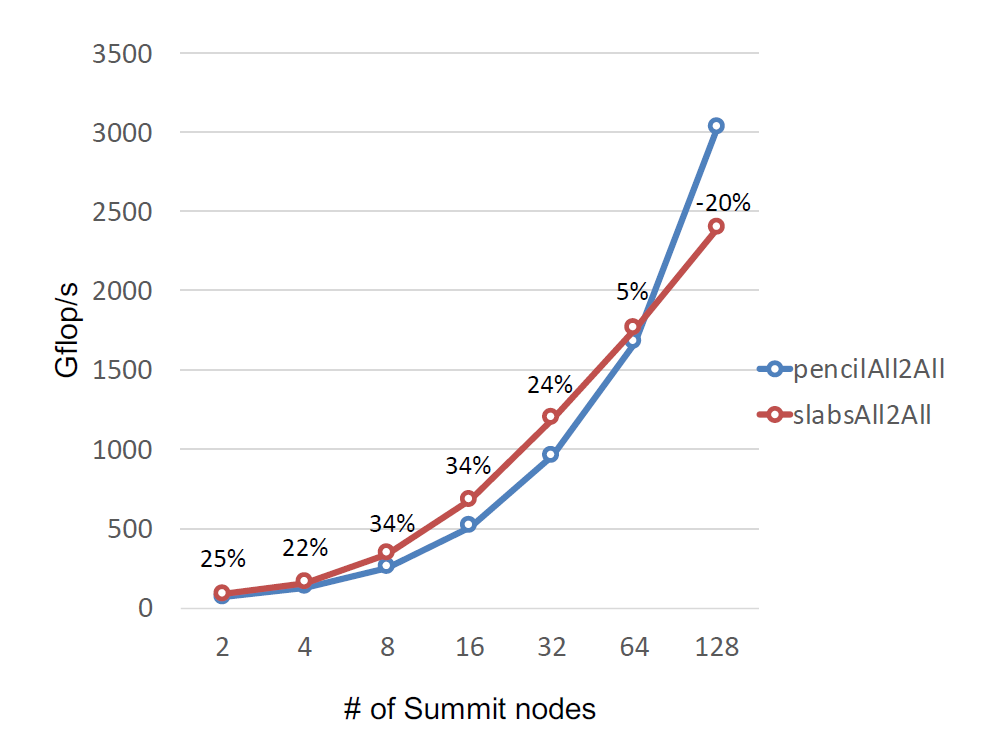
\includegraphics[width=0.7\linewidth, keepaspectratio]{../res/bench2.png}
		\footnotemark[1]
	\end{figure}
	Nachteil: Quadratischer Speicherverbrauch pro Knoten
	
\footnotetext[1]{\tiny Shajek H., Tomov S., Ayala A., Haidar A., Dongarra J:\\{\sl GPUDirect MPI Communications and Optimizations to Accelerate FFTs on Exascale Systems};\\EuroMPI ’19 Posters, September 11-13, 2019, Zurich, Switzerland}
}
\frame
{
	\frametitle{Ansatz 3}
	Dynamische Analysen hinsichtlich
	\begin{itemize}
		\item Speicherverbrauch
		\item Rechenlast
	\end{itemize}
	zur optimalen Auslastung und Aufteilung auf die Einheiten von Rechenressourcen 
	\begin{enumerate}
		\item{Knoten}
		\item{Sockel}
		\item{Prozessor}
	\end{enumerate}
	$\implies$ Vermeidung unnötiger Kommunikation.
}


\frame
{
	\begin{center}
		And that's all she wrote.\\
		\Large Vielen Dank für die Aufmerksamkeit! \normalsize\\
		\tiny Noch Fragen? \normalsize
	\end{center}
}

\end{document}
